\documentclass{beamer}

\pdfmapfile{+sansmathaccent.map}


\mode<presentation>
{
	\usetheme{Warsaw} % or try Darmstadt, Madrid, Warsaw, Rochester, CambridgeUS, ...
	\usecolortheme{seahorse} % or try seahorse, beaver, crane, wolverine, ...
	\usefonttheme{serif}  % or try serif, structurebold, ...
	\setbeamertemplate{navigation symbols}{}
	\setbeamertemplate{caption}[numbered]
} 


%%%%%%%%%%%%%%%%%%%%%%%%%%%%
% itemize settings

\definecolor{mypaleblue}{RGB}{240, 240, 255}
\definecolor{mylightblue}{RGB}{120, 150, 255}
\definecolor{myblue}{RGB}{90, 90, 255}
\definecolor{mygblue}{RGB}{70, 110, 240}
\definecolor{mydarkblue}{RGB}{0, 0, 180}
\definecolor{myblackblue}{RGB}{40, 40, 120}

\definecolor{mygreen}{RGB}{0, 200, 0}
\definecolor{mydarkgreen}{RGB}{0, 120, 0}
\definecolor{mygreen2}{RGB}{245, 255, 230}

\definecolor{mygray}{gray}{0.8}
\definecolor{mygray2}{RGB}{130, 130, 130}
\definecolor{mydarkgray}{RGB}{80, 80, 160}
\definecolor{mylightgray}{RGB}{160, 160, 160}

\definecolor{mydarkred}{RGB}{160, 30, 30}
\definecolor{mylightred}{RGB}{255, 150, 150}
\definecolor{myred}{RGB}{200, 110, 110}
\definecolor{myblackred}{RGB}{120, 40, 40}

\definecolor{mypink}{RGB}{255, 30, 80}
\definecolor{myhotpink}{RGB}{255, 80, 200}
\definecolor{mywarmpink}{RGB}{255, 60, 160}
\definecolor{mylightpink}{RGB}{255, 80, 200}
\definecolor{mydarkpink}{RGB}{155, 25, 60}

\definecolor{mydarkcolor}{RGB}{60, 25, 155}
\definecolor{mylightcolor}{RGB}{130, 180, 250}

\setbeamertemplate{itemize items}[default]

\setbeamertemplate{itemize item}{\color{myblackblue}$\blacksquare$}
\setbeamertemplate{itemize subitem}{\color{mydarkblue}$\blacktriangleright$}
\setbeamertemplate{itemize subsubitem}{\color{mygray}$\blacksquare$}

\setbeamercolor{palette quaternary}{fg=white,bg=mygblue} %mydarkgray
\setbeamercolor{titlelike}{parent=palette quaternary}

\setbeamercolor{palette quaternary2}{fg=white,bg=mygblue}%black myblue
\setbeamercolor{frametitle}{parent=palette quaternary2}

\setbeamerfont{frametitle}{size=\Large,series=\scshape}
\setbeamerfont{framesubtitle}{size=\normalsize,series=\upshape}


%%%%%%%%%%%%%%%%%%%%%%%%%%%%
% block settings

%\setbeamercolor{block title}{bg=red!50,fg=black}
%\setbeamercolor{block title}{bg=mylightblue,fg=black}
\setbeamercolor{block title}{bg=myblackblue,fg=white}

\setbeamercolor*{block title example}{bg=mygreen!40!white,fg=black}

\setbeamercolor*{block body example}{fg= black,
	bg= mygreen2}


%%%%%%%%%%%%%%%%%%%%%%%%%%%%
% URL settings
\hypersetup{
	colorlinks=false,
	linkcolor=blue,
	filecolor=blue,      
	urlcolor=blue,
}

%%%%%%%%%%%%%%%%%%%%%%%%%%

\renewcommand{\familydefault}{\rmdefault}

\usepackage{amsmath}
\usepackage{mathtools}

\usepackage{subcaption}

\usepackage{qrcode}

\newcommand{\bo}[1] {\mathbf{#1}}
\newcommand{\R}{\mathbb{R}} 
\newcommand{\T}{^\top}     



\newcommand{\mydate}{Spring 2025}

\newcommand{\mygit}{\textcolor{blue}{\href{https://github.com/SergeiSa/Computational-Intelligence-2025}{github.com/SergeiSa/Computational-Intelligence-2025}}}

\newcommand{\myqr}{ \textcolor{black}{\qrcode[height=1.5in]{https://github.com/SergeiSa/Computational-Intelligence-2025}}
}

\newcommand{\myqrframe}{
	\begin{frame}
		\centerline{Lecture slides are available via Github, links are on Moodle:}
		\bigskip
		\centerline{\mygit}
		\bigskip
		\myqr
	\end{frame}
}


\newcommand{\bref}[2] {\textcolor{blue}{\href{#1}{#2}}}



%%%%%%%%%%%%%%%%%%%%%%%%%%%%
% code settings

\usepackage{listings}
\usepackage{color}
% \definecolor{mygreen}{rgb}{0,0.6,0}
% \definecolor{mygray}{rgb}{0.5,0.5,0.5}
\definecolor{mymauve}{rgb}{0.58,0,0.82}
\lstset{ 
	backgroundcolor=\color{white},   % choose the background color; you must add \usepackage{color} or \usepackage{xcolor}; should come as last argument
	basicstyle=\footnotesize,        % the size of the fonts that are used for the code
	breakatwhitespace=false,         % sets if automatic breaks should only happen at whitespace
	breaklines=true,                 % sets automatic line breaking
	captionpos=b,                    % sets the caption-position to bottom
	commentstyle=\color{mygreen},    % comment style
	deletekeywords={...},            % if you want to delete keywords from the given language
	escapeinside={\%*}{*)},          % if you want to add LaTeX within your code
	extendedchars=true,              % lets you use non-ASCII characters; for 8-bits encodings only, does not work with UTF-8
	firstnumber=0000,                % start line enumeration with line 0000
	frame=single,	                   % adds a frame around the code
	keepspaces=true,                 % keeps spaces in text, useful for keeping indentation of code (possibly needs columns=flexible)
	keywordstyle=\color{blue},       % keyword style
	language=Octave,                 % the language of the code
	morekeywords={*,...},            % if you want to add more keywords to the set
	numbers=left,                    % where to put the line-numbers; possible values are (none, left, right)
	numbersep=5pt,                   % how far the line-numbers are from the code
	numberstyle=\tiny\color{mygray}, % the style that is used for the line-numbers
	rulecolor=\color{black},         % if not set, the frame-color may be changed on line-breaks within not-black text (e.g. comments (green here))
	showspaces=false,                % show spaces everywhere adding particular underscores; it overrides 'showstringspaces'
	showstringspaces=false,          % underline spaces within strings only
	showtabs=false,                  % show tabs within strings adding particular underscores
	stepnumber=2,                    % the step between two line-numbers. If it's 1, each line will be numbered
	stringstyle=\color{mymauve},     % string literal style
	tabsize=2,	                   % sets default tabsize to 2 spaces
	title=\lstname                   % show the filename of files included with \lstinputlisting; also try caption instead of title
}

%%%%%%%%%%%%%%%%%%%%%%%%%%%%
% tikz settings

\usepackage{tikz}
\tikzset{every picture/.style={line width=0.75pt}}

%%%%%%%%%%%%%%%%%%%%%%%%%%%%




\title{Mixed Integer Convex Programming}
\subtitle{Computational Intelligence, Lecture 12}
\author{by Sergei Savin}
\centering
\date{\mydate}


\begin{document}
\maketitle


\begin{frame}{Content}

\begin{itemize}
\item Mixed Integer Linear Programming (MILP)
\item Mixed Integer Quadratic Programming (MIQP)
\item Example: Footstep planning
\item Big-M method relaxation
\item Example: switching control
\item Homework
\end{itemize}

\end{frame}



\begin{frame}{Mixed Integer Linear Programming (MILP)}
%\framesubtitle{General form}
\begin{flushleft}

A general form of a mixed-integer linear program is:

%
\begin{equation} \label{LP}
\begin{aligned}
& \underset{\mathbf{x}}{\text{minimize}}
& & \mathbf{f}^\top \mathbf{x}, \\
& \text{subject to}
& & \begin{cases} 
\mathbf{A} \mathbf{x}
\leq 
\mathbf{b}, \\ 
\mathbf{C}\mathbf{x} = 
\mathbf{d},  \\
\mathbf{x}_1, ..., \mathbf{x}_m \in \mathbb{R},\\
\mathbf{x}_{m+1}, ..., \mathbf{x}_n \in \mathbb{N}.
\end{cases}
%
\end{aligned}
\end{equation}
 
In other words, the only difference is that some of the variables are only allowed to assume pure integer values.
 
\end{flushleft}
\end{frame}



\begin{frame}{Mixed Integer Convex Programming (MICP)}
%\framesubtitle{General form}
\begin{flushleft}

A general form of a mixed-integer convex program is:

%
\begin{equation} \label{QP}
\begin{aligned}
& \underset{\mathbf{x}}{\text{minimize}}
& & 
l(\mathbf{x}) \ \ \ \ \textcolor{mylightgray}{\text{convex cost}} \\
& \text{subject to}
& & \begin{cases} 
g(\mathbf{x}) \leq 0, &\ \ \ \ \textcolor{mylightgray}{\text{convex domain}} \\ 
\mathbf{C}\mathbf{x} = 
\mathbf{d},  &\\
x_1, ..., x_m \in \mathbb{R}, &\ \ \ \ \textcolor{mylightgray}{\text{continuous variables}}\\
x_{m+1}, ..., x_n \in \mathbb{N}. &\ \ \ \ \textcolor{mylightgray}{\text{integer variables}}
\end{cases}
%
\end{aligned}
\end{equation}
 
\end{flushleft}
\end{frame}



\begin{frame}{Remarks}
% \framesubtitle{General form}
\begin{flushleft}

\begin{itemize}
    \item Mixed-integer convex programs are not convex, even if the name seems to suggest otherwise. 
    \item The "convex program" in the phrase "mixed-integer convex program" should be understood as "if we fix values of the integer variables, or relax them into reals, the result will be a convex program".
    \item Mixed integer programs are usually solved using \emph{branch and bound algorithms}; in worse case scenario, the algorithms performs exhaustive search.
    \item In robotics applications, integer variables in mixed integer programs are often restricted to binary values, i.e. $\mathbf{y} \in \{0, 1\}^n.$. It is still called "mixed-integer" in the literature, although phrases such as "mixed-binary" or "binary constraints" are not rare.
\end{itemize}
 
\end{flushleft}
\end{frame}



\begin{frame}{Example: Footstep planning}
\framesubtitle{Problem statement}
\begin{flushleft}

Given $N$ convex regions defined by linear inequalities $\{ \mathbf{x}: \  \mathbf{A}_i \mathbf{x} \leq \mathbf{b}_i \}$ (which is called H-polytope representation), find a sequence of $K$ points (footsteps) from the given starting point to the given goal point, such that all footsteps lie in one of the convex regions.

\begin{equation}
\begin{aligned}
& \underset{\mathbf{x}_1, \ ..., \ \mathbf{x}_K}{\text{minimize}}
& & ||\mathbf{x}_1 - \mathbf{x}_{\text{start}}|| + ||\mathbf{x}_K - \mathbf{x}_{\text{goal}}||, \\
& \text{subject to}
& & \exists \{ \mathbf{A}_j, \mathbf{b}_j\} \in \Omega \ \text{s.t.} \ \mathbf{A}_j\mathbf{x}_i \leq \mathbf{b}_j
\end{aligned}
\end{equation}

\bigskip

where $\Omega = \{ \{ \mathbf{A}_1, \mathbf{b}_1\}, \ \{ \mathbf{A}_2, \mathbf{b}_2\}, \ ..., \ \{ \mathbf{A}_N, \mathbf{b}_N\} \}$. This is not a convex program.
 
\end{flushleft}
\end{frame}




\begin{frame}{Big-M method, 1}
%\framesubtitle{Basic idea}
\begin{flushleft}


One of the key methods associated with the use of mixed-integer programming in robotics is the big-M method. 

\bigskip

Assume you have two inequalities, $\mathbf{a}_1^\top \mathbf{x} \leq b_1$ and $\mathbf{a}_2^\top \mathbf{x} \leq b_2$, and you are happy if at least one of them holds. Define a new binary variables $c_1, c_2 \in \{0, \ 1 \}$ and find a big enough constant $M$, such that $\mathbf{a}_1^\top \mathbf{x} \leq b_1 + M$ and $\mathbf{a}_2^\top \mathbf{x} \leq b_2 + M$ holds for all of your domain (of the part of it you are interested in).



\begin{figure} [h!]
	\begin{center}
		
\tikzset{every picture/.style={line width=0.75pt}} %set default line width to 0.75pt        

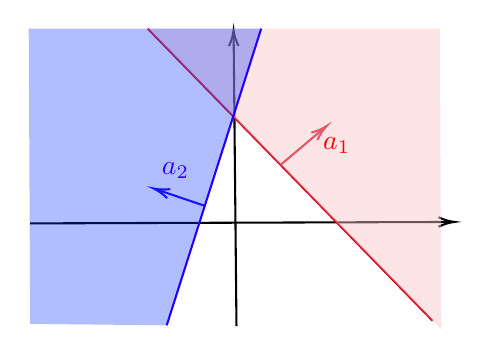
\begin{tikzpicture}[x=0.75pt,y=0.75pt,yscale=-0.7,xscale=0.7]
	%uncomment if require: \path (0,300); %set diagram left start at 0, and has height of 300
	
	%Straight Lines [id:da8513797768325038] 
	\draw    (18.43,141) -- (308.43,140.01) ;
	\draw [shift={(310.43,140)}, rotate = 179.8] [color={rgb, 255:red, 0; green, 0; blue, 0 }  ][line width=0.75]    (10.93,-3.29) .. controls (6.95,-1.4) and (3.31,-0.3) .. (0,0) .. controls (3.31,0.3) and (6.95,1.4) .. (10.93,3.29)   ;
	%Straight Lines [id:da7015285035770829] 
	\draw    (160.43,211.71) -- (158.45,10) ;
	\draw [shift={(158.43,8)}, rotate = 89.44] [color={rgb, 255:red, 0; green, 0; blue, 0 }  ][line width=0.75]    (10.93,-3.29) .. controls (6.95,-1.4) and (3.31,-0.3) .. (0,0) .. controls (3.31,0.3) and (6.95,1.4) .. (10.93,3.29)   ;
	%Straight Lines [id:da2713141928527276] 
	\draw [color={rgb, 255:red, 208; green, 2; blue, 27 }  ,draw opacity=1 ]   (190.43,101) -- (220.9,75.29) ;
	\draw [shift={(222.43,74)}, rotate = 139.84] [color={rgb, 255:red, 208; green, 2; blue, 27 }  ,draw opacity=1 ][line width=0.75]    (10.93,-3.29) .. controls (6.95,-1.4) and (3.31,-0.3) .. (0,0) .. controls (3.31,0.3) and (6.95,1.4) .. (10.93,3.29)   ;
	%Straight Lines [id:da5353768254567948] 
	\draw [color={rgb, 255:red, 208; green, 2; blue, 27 }  ,draw opacity=1 ]   (99.43,7) -- (295.43,208) ;
	%Shape: Polygon [id:ds8045398869675415] 
	\draw  [draw opacity=0][fill={rgb, 255:red, 253; green, 195; blue, 195 }  ,fill opacity=0.44 ] (300.43,7) -- (301.43,214) -- (99.43,7) -- cycle ;
	%Shape: Polygon [id:ds20123771866467055] 
	\draw  [draw opacity=0][fill={rgb, 255:red, 1; green, 44; blue, 255 }  ,fill opacity=0.31 ] (177.43,7) -- (112.43,211.14) -- (18.43,210.14) -- (17.43,7) -- cycle ;
	%Straight Lines [id:da13860340047318598] 
	\draw [color={rgb, 255:red, 22; green, 20; blue, 255 }  ,draw opacity=1 ]   (138.93,129) -- (105.32,117.64) ;
	\draw [shift={(103.43,117)}, rotate = 18.68] [color={rgb, 255:red, 22; green, 20; blue, 255 }  ,draw opacity=1 ][line width=0.75]    (10.93,-3.29) .. controls (6.95,-1.4) and (3.31,-0.3) .. (0,0) .. controls (3.31,0.3) and (6.95,1.4) .. (10.93,3.29)   ;
	%Straight Lines [id:da9081216075039891] 
	\draw [color={rgb, 255:red, 34; green, 0; blue, 255 }  ,draw opacity=1 ]   (177.43,7) -- (112.43,211.14) ;
	
	% Text Node
	\draw (218,80) node [anchor=north west][inner sep=0.75pt]  [color={rgb, 255:red, 255; green, 0; blue, 0 }  ,opacity=1 ] [align=left] {$\displaystyle a_{1}$};
	% Text Node
	\draw (107,97) node [anchor=north west][inner sep=0.75pt]  [color={rgb, 255:red, 46; green, 0; blue, 255 }  ,opacity=1 ] [align=left] {$\displaystyle a_{2}$};
	
	
\end{tikzpicture}
	\end{center} 
\end{figure}

\end{flushleft}
\end{frame}



\begin{frame}{Big-M method, 2}
	%\framesubtitle{Basic idea}
	\begin{flushleft}
		
		Let us put the following constraint on the variables $c_1$, $c_2$:
		%
		\begin{equation}
			c_1 + c_2 = 1
		\end{equation}
		
		The pair of variables $(c_1, c_2)$ together can assume only two values - (1, 0) and (0, 1). We can modify the inequalities $\mathbf{a}_1\T \mathbf{x} \leq b_1$ and $\mathbf{a}_2\T \mathbf{x} \leq b_2$:
		%
		\begin{equation}
			\begin{cases}
				\mathbf{a}_1^\top \mathbf{x} \leq b_1 + M \cdot c_1 \\
				\mathbf{a}_2^\top \mathbf{x} \leq b_2 + M \cdot c_2
			\end{cases}
		\end{equation}
		
		If $(c_1, c_2) = (1, 0)$, then modified inequalities become:
		%
		\begin{equation}
			\begin{cases}
				\textcolor{mydarkgray}{ \mathbf{a}_1\T \mathbf{x} \leq b_1 + M }  
				\ & \textcolor{mygray}{\text{- true for all }  \mathbf{x}}
				\\
				\mathbf{a}_2^\top \mathbf{x} \leq b_2 
				\ & \textcolor{mygray}{\text{- original constraint } }
			\end{cases}
		\end{equation}
		
		 
		 If $(c_1, c_2) = (0, 1)$, then modified inequalities become:
		 %
		 \begin{equation}
		 	\begin{cases}
		 		\mathbf{a}_1\T \mathbf{x} \leq b_1  
		 		\ & \textcolor{mygray}{\text{- original constraint } }
		 		\\
		 		\textcolor{mydarkgray}{\mathbf{a}_2^\top \mathbf{x} \leq b_2  + M}
		 		\ & \textcolor{mygray}{\text{- true for all }  \mathbf{x}}
		 	\end{cases}
		 \end{equation}
		
		
		
	\end{flushleft}
\end{frame}



\begin{frame}{Big-M method, 3}
	%\framesubtitle{Basic idea}
	\begin{flushleft}
		
		With that, we propose the following constraint:
		
		\begin{equation}
			\begin{cases}
				\mathbf{a}_1^\top \mathbf{x} \leq b_1 + M \cdot c_1 \\
				\mathbf{a}_2^\top \mathbf{x} \leq b_2 + M \cdot c_2 \\
				c_1 + c_2 = 1  \\
				c_i  \in \{0, \ 1 \}
			\end{cases}
		\end{equation}
		
		
		\begin{figure} [h!]
			\begin{center}
				


\tikzset{every picture/.style={line width=0.75pt}} %set default line width to 0.75pt        

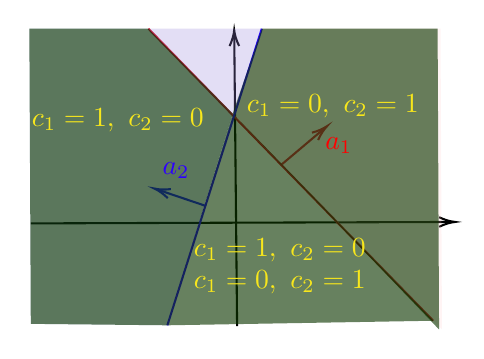
\begin{tikzpicture}[x=0.75pt,y=0.75pt,yscale=-0.7,xscale=0.7]
	%uncomment if require: \path (0,300); %set diagram left start at 0, and has height of 300
	
	%Straight Lines [id:da043120004745246465] 
	\draw    (18.43,141) -- (308.43,140.01) ;
	\draw [shift={(310.43,140)}, rotate = 179.8] [color={rgb, 255:red, 0; green, 0; blue, 0 }  ][line width=0.75]    (10.93,-3.29) .. controls (6.95,-1.4) and (3.31,-0.3) .. (0,0) .. controls (3.31,0.3) and (6.95,1.4) .. (10.93,3.29)   ;
	%Straight Lines [id:da10089229777665709] 
	\draw    (160.43,211.71) -- (158.45,10) ;
	\draw [shift={(158.43,8)}, rotate = 89.44] [color={rgb, 255:red, 0; green, 0; blue, 0 }  ][line width=0.75]    (10.93,-3.29) .. controls (6.95,-1.4) and (3.31,-0.3) .. (0,0) .. controls (3.31,0.3) and (6.95,1.4) .. (10.93,3.29)   ;
	%Straight Lines [id:da7268273424354579] 
	\draw [color={rgb, 255:red, 208; green, 2; blue, 27 }  ,draw opacity=1 ]   (190.43,101) -- (220.9,75.29) ;
	\draw [shift={(222.43,74)}, rotate = 139.84] [color={rgb, 255:red, 208; green, 2; blue, 27 }  ,draw opacity=1 ][line width=0.75]    (10.93,-3.29) .. controls (6.95,-1.4) and (3.31,-0.3) .. (0,0) .. controls (3.31,0.3) and (6.95,1.4) .. (10.93,3.29)   ;
	%Straight Lines [id:da5256799633351579] 
	\draw [color={rgb, 255:red, 208; green, 2; blue, 27 }  ,draw opacity=1 ]   (99.43,7) -- (295.43,208) ;
	%Shape: Polygon [id:ds16795660112353028] 
	\draw  [draw opacity=0][fill={rgb, 255:red, 253; green, 195; blue, 195 }  ,fill opacity=0.19 ] (300.43,7) -- (301.43,214) -- (99.43,7) -- cycle ;
	%Shape: Polygon [id:ds657177688701895] 
	\draw  [draw opacity=0][fill={rgb, 255:red, 1; green, 44; blue, 255 }  ,fill opacity=0.11 ] (177.43,7) -- (112.43,211.14) -- (18.43,210.14) -- (17.43,7) -- cycle ;
	%Straight Lines [id:da523733379699233] 
	\draw [color={rgb, 255:red, 22; green, 20; blue, 255 }  ,draw opacity=1 ]   (138.93,129) -- (105.32,117.64) ;
	\draw [shift={(103.43,117)}, rotate = 18.68] [color={rgb, 255:red, 22; green, 20; blue, 255 }  ,draw opacity=1 ][line width=0.75]    (10.93,-3.29) .. controls (6.95,-1.4) and (3.31,-0.3) .. (0,0) .. controls (3.31,0.3) and (6.95,1.4) .. (10.93,3.29)   ;
	%Straight Lines [id:da5166718561288546] 
	\draw [color={rgb, 255:red, 34; green, 0; blue, 255 }  ,draw opacity=1 ]   (177.43,7) -- (112.43,211.14) ;
	%Shape: Polygon [id:ds9146954261231561] 
	\draw  [draw opacity=0][fill={rgb, 255:red, 14; green, 55; blue, 1 }  ,fill opacity=0.64 ] (99.43,7) -- (157.43,65.43) -- (148.58,94.07) -- (112.43,211.14) -- (18.43,210.14) -- (17.43,7) -- cycle ;
	%Shape: Polygon [id:ds7825723532393902] 
	\draw  [draw opacity=0][fill={rgb, 255:red, 14; green, 55; blue, 1 }  ,fill opacity=0.63 ] (298.43,7) -- (298.84,92.02) -- (299.43,214) -- (157.43,65.43) -- (177.43,7) -- cycle ;
	%Shape: Polygon [id:ds09269151620752769] 
	\draw  [draw opacity=0][fill={rgb, 255:red, 14; green, 55; blue, 1 }  ,fill opacity=0.63 ] (295.43,208) -- (112.43,211.14) -- (157.43,65.43) -- cycle ;
	
	% Text Node
	\draw (219,80) node [anchor=north west][inner sep=0.75pt]  [color={rgb, 255:red, 255; green, 0; blue, 0 }  ,opacity=1 ] [align=left] {$\displaystyle a_{1}$};
	% Text Node
	\draw (107,97) node [anchor=north west][inner sep=0.75pt]  [color={rgb, 255:red, 46; green, 0; blue, 255 }  ,opacity=1 ] [align=left] {$\displaystyle a_{2}$};
	% Text Node
	\draw (165,50) node [anchor=north west][inner sep=0.75pt]  [color={rgb, 255:red, 248; green, 231; blue, 28 }  ,opacity=1 ] [align=left] {$\displaystyle c_{1} =0,\ c_{2} =1$};
	% Text Node
	\draw (17,60) node [anchor=north west][inner sep=0.75pt]  [color={rgb, 255:red, 248; green, 231; blue, 28 }  ,opacity=1 ] [align=left] {$\displaystyle c_{1} =1,\ c_{2} =0$};
	% Text Node
	\draw (128.51,149.6) node [anchor=north west][inner sep=0.75pt]  [color={rgb, 255:red, 248; green, 231; blue, 28 }  ,opacity=1 ] [align=left] {$\displaystyle c_{1} =1,\ c_{2} =0$};
	% Text Node
	\draw (128.51,171.6) node [anchor=north west][inner sep=0.75pt]  [color={rgb, 255:red, 248; green, 231; blue, 28 }  ,opacity=1 ] [align=left] {$\displaystyle c_{1} =0,\ c_{2} =1$};
	
	
\end{tikzpicture}

			\end{center} 
		\end{figure}
		
	\end{flushleft}
\end{frame}




\begin{frame}{Choosing between polytopes, 1}
%\framesubtitle{Systems of inequalities}
\begin{flushleft}

It works the same way for the case when you have three (or two or more) systems of inequalities $\mathbf{A}_1 \mathbf{x} \leq \mathbf{b}_1$, $\mathbf{A}_2 \mathbf{x} \leq \mathbf{b}_2$, $\mathbf{A}_3 \mathbf{x} \leq \mathbf{b}_3$ and are happy if at least one holds:

\begin{equation}
    \begin{cases}
    \mathbf{A}_1 \mathbf{x} \leq \mathbf{b}_1 + M \cdot \mathbf{1} \cdot (1 - c_1) \\
    \mathbf{A}_2 \mathbf{x} \leq \mathbf{b}_2 + M \cdot \mathbf{1} \cdot (1 - c_2) \\
    \mathbf{A}_3 \mathbf{x} \leq \mathbf{b}_3 + M \cdot \mathbf{1} \cdot (1 - c_3) \\
    c_1 + c_2 + c_3 = 1 \\
    c_i  \in \{0, \ 1 \}
    \end{cases}
\end{equation}

where $\mathbf{1}$ is a vector of all ones. Notice that constraint $c_1 + c_2 + c_3 = 1$ can be replaced with $c_1 + c_2 + c_3 >= 1$, allowing avoid relaxing more than one region.

\end{flushleft}
\end{frame}



\begin{frame}{Choosing between polytopes, 2}
%\framesubtitle{Illustration, part 1}
\begin{flushleft}

Below are two H-polytops (convex regions represented by systems of inequalities):

\begin{figure} [h!]
\begin{center}
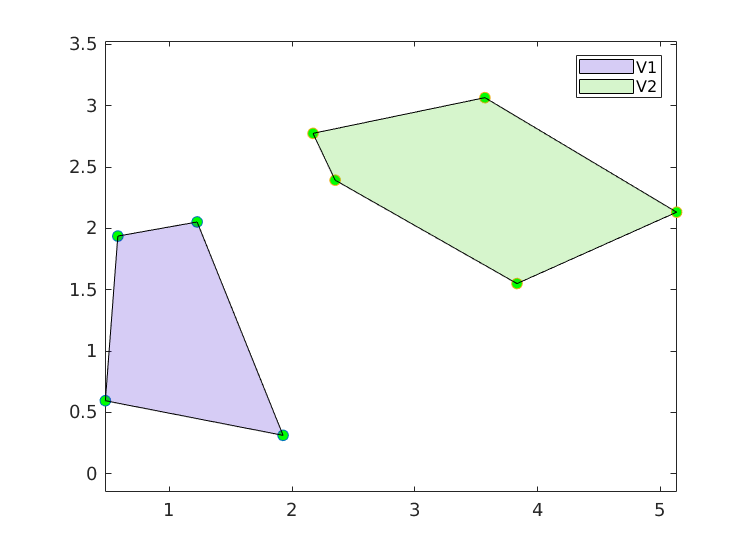
\includegraphics[width=2.6in]{fig1.png}
\end{center} 
% \caption{AR 601 bipedal robot, Innopolis University}
\end{figure}

As we can see, their union represents a non-convex domain, and they have no intersection.

\end{flushleft}
\end{frame}


\begin{frame}{Choosing between polytopes, 3}
%\framesubtitle{Illustration, part 2}
\begin{flushleft}

Now, one of them is relaxed as described above. Notice that the intersection of the two polytopes is non-relaxed polytope. 

\begin{figure}
\centering
\begin{subfigure}{.5\textwidth}
  \centering
  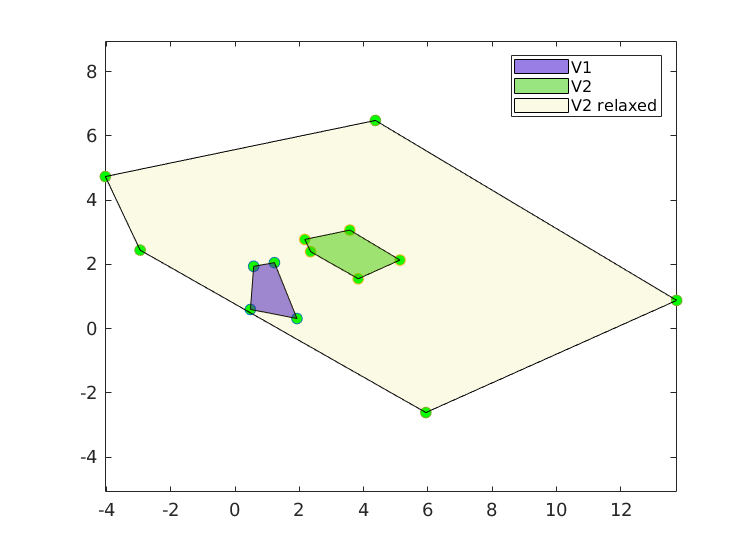
\includegraphics[width=1.1\linewidth]{fig2.png}
%   \caption{Simplified model}
\end{subfigure}%
\begin{subfigure}{.5\textwidth}
  \centering
  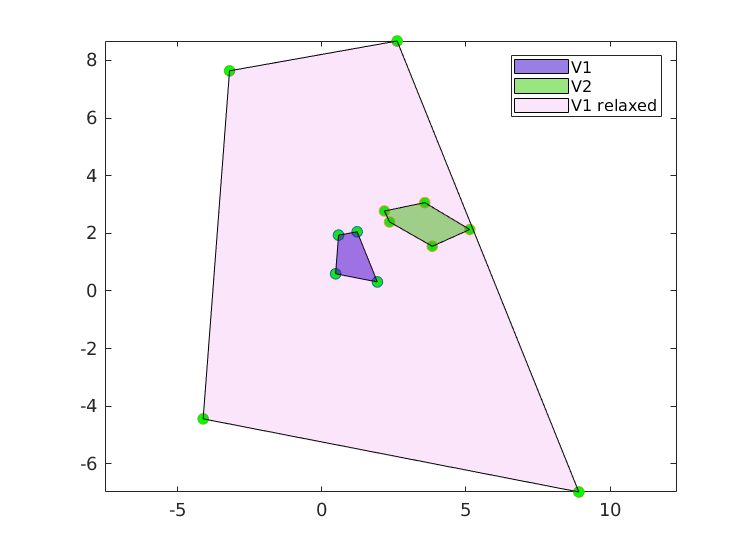
\includegraphics[width=1.1\linewidth]{fig3.png}
%   \caption{Simplified model}
\end{subfigure}
\end{figure}

\end{flushleft}
\end{frame}


\begin{frame}{Choosing between polytopes, 4}
\framesubtitle{Multiple variables}
\begin{flushleft}

If you have multiple variables $\mathbf{x}_1$, ..., $\mathbf{x}_K$, and each should belong to at least one of the H-polytopes $\{ \mathbf{A}_i, \mathbf{b}_i\}$, this can also be represented using big-M method:

\begin{equation}
    \begin{cases}
    \mathbf{A}_1 \mathbf{x}_k \leq \mathbf{b}_1 + M \cdot \mathbf{1} \cdot (1 - c_{1, k}) \\
    \mathbf{A}_2 \mathbf{x}_k \leq \mathbf{b}_2 + M \cdot \mathbf{1} \cdot (1 - c_{2, k}) \\
    \mathbf{A}_3 \mathbf{x}_k \leq \mathbf{b}_3 + M \cdot \mathbf{1} \cdot (1 - c_{3, k}) \\
    c_{1, k} + c_{2, k} + c_{3, k} = 1 \\
    c_{i, k}  \in \{0, \ 1 \} \\
    k = 1,...,K
    \end{cases}
\end{equation}

Notice that the only difference from the previous example is that now we have $K$ sets of binary variables $c_{1, k}$,  $c_{2, k}$ and $c_{3, k}$.

\end{flushleft}
\end{frame}






\begin{frame}{Example: Footstep planning}
\framesubtitle{Formulation as MIQP}
\begin{flushleft}

Using big-M relaxation we can now formulate the problem as follows:

\begin{equation}
\begin{aligned}
& \underset{\mathbf{x}_k, \ \mathbf{c}_{i,k}}{\text{minimize}}
& & ||\mathbf{x}_1 - \mathbf{x}_{\text{start}}|| + ||\mathbf{x}_K - \mathbf{x}_{\text{goal}}||, \\
& \text{subject to}
& & \begin{cases}
    \mathbf{A}_i \mathbf{x}_k \leq \mathbf{b}_i + M \cdot \mathbf{1} \cdot (1 - c_{i, k}), \ i = 1,...,N \\
    \sum_{i=1}^N c_{i, k} = 1 \\
    c  \in \{0, \ 1 \}^{N, \ K} \\
    k = 1,...,K
    \end{cases}
\end{aligned}
\end{equation}

 
\end{flushleft}
\end{frame}





\begin{frame}{Example: Footstep planning}
\framesubtitle{Evenly spaced steps}
\begin{flushleft}

In order to make the footsteps evenly spaced we add cost on the distance between consequent steps:

\begin{equation*}
\begin{aligned}
& \underset{\mathbf{x}_k, \ \mathbf{c}_{i,k}}{\text{minimize}}
& & ||\mathbf{x}_1 - \mathbf{x}_{\text{start}}||^2 + ||\mathbf{x}_K - \mathbf{x}_{\text{goal}}||^2 + w \cdot \sum_{k=1}^{K-1} ||\mathbf{x}_{i+1} - \mathbf{x}_i||^2, \\
& \text{subject to}
& & \begin{cases}
    \mathbf{A}_i \mathbf{x}_k \leq \mathbf{b}_i + M \cdot \mathbf{1} \cdot (1 - c_{i, k}), \ i = 1,...,N \\
    \sum_{i=1}^N c_{i, k} = 1 \\
    c  \in \{0, \ 1 \}^{N, \ K} \\
    k = 1,...,K
    \end{cases}
\end{aligned}
\end{equation*}

where $w$ is a weight, a coefficient we can tune to adjust relative importance of our primary objective (starting from the point $\mathbf{x}_{\text{start}}$ and finishing at the point $\mathbf{x}_{\text{goal}}$ and our secondary objective (making the footsteps evenly spaced).  
 
\end{flushleft}
\end{frame}




\begin{frame}{Example: Footstep planning}
\framesubtitle{Code, part 1}
\begin{flushleft}

\begin{lstlisting}[language=Matlab]
n = 7; A = randn(n, n) - 3*rand*eye(n);
Q = eye(n);

cvx_begin sdp
    variable P(n, n) symmetric
    minimize 0
    subject to
        P >= 0;
        A'*P + P*A + Q <= 0;
cvx_end

if strcmp(cvx_status, 'Solved')
    [eig(A), eig(A*P + P*A' + Q), eig(P)]
else
    eig(A)
end
\end{lstlisting}
 
\end{flushleft}
\end{frame}


\begin{frame}{Example: Footstep planning}
\framesubtitle{Code, part 2}
\begin{flushleft}

\begin{lstlisting}[language=Matlab]
n = 7; A = 0.35*randn(n, n);
Q = eye(n);

cvx_begin sdp
    variable P(n, n) symmetric
    minimize 0
    subject to
        P >= 0;
        A'*P*A - P + Q <= 0;
cvx_end

if strcmp(cvx_status, 'Solved')
    [abs(eig(A)), eig(A'*P*A - P), eig(P)]
else
    abs(eig(A))
end
\end{lstlisting}
 
\end{flushleft}
\end{frame}




\begin{frame}{Example: switching control}
	\framesubtitle{Multiple variables}
	\begin{flushleft}
		
		Consider the case when you have a control system $\dot{\bo{x}} =\bo{A}\bo{x} + \bo{B}_1\bo{u}_1 + \bo{B}_2\bo{u}_2$, but you are required to use either $\bo{B}_1\bo{u}_1$ or $\bo{B}_2\bo{u}_2$ at any time, not both.
		
		\bigskip
		
		This can be cast as a mixed-integer constraint:
		
		\begin{equation}
			\begin{cases}
				||\bo{u}_1|| \leq M (1 - c_1) \\
				||\bo{u}_2|| \leq M (1 - c_2) \\
				c_1 + c_2 = 1
			\end{cases}
		\end{equation}
		
	\end{flushleft}
\end{frame}




\begin{frame}{Homework}
% \framesubtitle{Parameter estimation}
\begin{flushleft}

Implement footstep planning for a biped, making sure every pair of steps lands in the same H-polytope.

\end{flushleft}
\end{frame}



\myqrframe

\end{document}
